\begin{figure}[h]
	\centering
	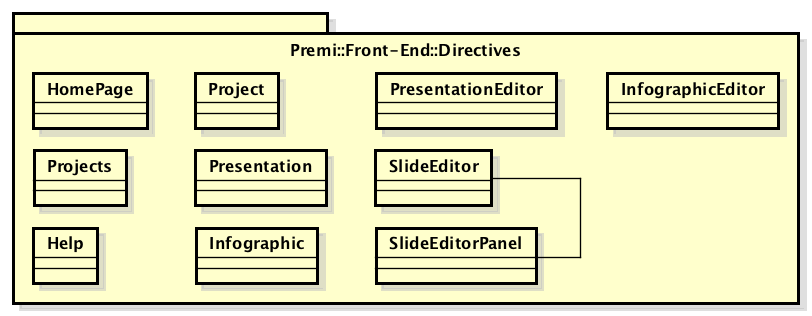
\includegraphics[width=0.7\linewidth]{img/premi_front_end_directives}
	\caption[Premi::Front-End::Directives]{Premi::Front-End::Directives}
\end{figure}
Il package gestisce le direttive del \gls{front-end}. Comunica con le view e con i controller per associarli nel giusto ordine e farli comunicare.
Per brevità nell'identificare una direttiva è stata omessa la dicitura Premi::\gls{Front-End}::Directives lasciando solamente il nome della direttiva stessa. Si assume dunque che la dicitura compatta <nomeDirettiva> rappresenta la forma estesa Premi::\gls{Front-End}::Directives::<nomeDirettiva>.
\newpage


\subsubsection{Help}
	\begin{figure}[h]
		\centering
		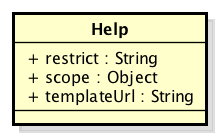
\includegraphics[width=0.4\linewidth]{img/premi_front_end_directives_help}
		\caption[Premi::Front-End::Directives::Help]{Premi::Front-End::Directives::Help}
	\end{figure}
	
	\paragraph{Descrizione}
	Rappresenta il componente grafico che permette di visualizzare gli aiuti agli utenti nelle varie sezioni dell'applicazione.
	
	\paragraph{Utilizzo}
	Viene utilizzata per consentire di far mostrare all'utente i tips nelle sezioni dell'applicazione. Si attiva a seconda dell'opzione selezionata dall'utente, se abilita l'aiuto all'uso dell'applicazione oppure no.
	
	\paragraph{Attributi}
	\begin{itemize}
		\item \textbf{+ controller: String}:\\
			Stringa che specifica il controller da associare alla direttiva. Per questa direttiva è l'\textit{HelpCtrl};
		\item \textbf{+ restrict: String}:\\
			Stringa che specifica la modalità con la quale è possibile inserire la direttiva all'interno della pagina;
		\item \textbf{+ scope: Object}:\\
			Oggetto scope locale della direttiva;
		\item \textbf{+ templateUrl: String}:\\
			Stringa che specifica il percordo dove è situato il file \gls{HTML} che contiene il \gls{template} della direttiva
	\end{itemize}
\newpage


\subsubsection{HomePage}
	\begin{figure}[h]
		\centering
		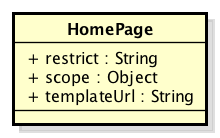
\includegraphics[width=0.4\linewidth]{img/premi_front_end_directives_homepage}
		\caption[Premi::Front-End::Directives::HomePage]{Premi::Front-End::Directives::HomePage}
	\end{figure}
	
	\paragraph{Descrizione}
	Rappresenta il componente grafico che permette all'utente di accedere alle sezioni di login e registrazione e per effettuare la ricerca. Questo componente è visibile all'apertura dell'applicazione.
	
	\paragraph{Utilizzo}
	Viene utilizzata per consentire all'utente di raggiungere le principali sezioni dell'applicazione e per eseguire la ricerca dei progetti. Deve essere inserita nella pagina iniziale del sito e deve essere attivata all'apertura dell'applicazione o nel momento in cui si deve effettuare una ricerca.
		
	\paragraph{Attributi}
	\begin{itemize}
		\item \textbf{+ controller: String}:\\
			Stringa che specifica il controller da associare alla direttiva. Per questa direttiva è l'\textit{HomePageCtrl};
		\item \textbf{+ restrict: String}:\\
			Stringa che specifica la modalità con la quale è possibile inserire la direttiva all'interno della pagina;
		\item \textbf{+ scope: Object}:\\
			Oggetto scope locale della direttiva;
		\item \textbf{+ templateUrl: String}:\\
			Stringa che specifica il percordo dove è situato il file \gls{HTML} che contiene il \gls{template} della direttiva
	\end{itemize}
\newpage
	
	
\subsubsection{InfographicEditor}
	\begin{figure}[h]
		\centering
		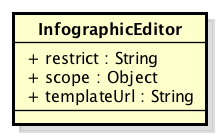
\includegraphics[width=0.4\linewidth]{img/premi_front_end_directives_infographiceditor}
		\caption[Premi::Front-End::Directives::InfographicEditor]{Premi::Front-End::Directives::InfographicEditor}
	\end{figure}
	
	\paragraph{Descrizione}
		Rappresenta il componente grafico che permette all'utente di accedere alla sezione per la gestione delle infografiche di un progetto.
	
	\paragraph{Utilizzo}
	Viene utilizzata per consentire all'utente di gestire le proprie infografiche, visualizzarle, modificarle e crearne di nuove. Deve essere inserita nella pagina relativa ai progetti di un utente e attivata quando è selezionata un'\gls{infografica} dalla pagina stessa.
	
	\paragraph{Attributi}
	\begin{itemize}
		\item \textbf{+ controller: String}:\\
			Stringa che specifica il controller da associare alla direttiva. Per questa classe èl'\textit{InfographicCtrl};
		\item \textbf{+ restrict: String}:\\
			Stringa che specifica la modalità con la quale è possibile inserire la direttiva all'interno della pagina;
		\item \textbf{+ scope: Object}:\\
			Oggetto scope locale della direttiva;
		\item \textbf{+ templateUrl: String}:\\
			Stringa che specifica il percordo dove è situato il file \gls{HTML} che contiene il \gls{template} della direttiva
	\end{itemize}
\newpage	
	

\subsubsection{Presentation}
	\begin{figure}[h]
		\centering
		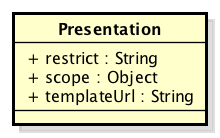
\includegraphics[width=0.4\linewidth]{img/premi_front_end_directives_presentation}
		\caption[Premi::Front-End::Directives::Presentation]{Premi::Front-End::Directives::Presentation}
	\end{figure}
	
	\paragraph{Descrizione}
	Rappresenta il componente grafico che permette all'utente di accedere alla sezione per la visualizzazione di una presentazione.
	
	\paragraph{Utilizzo}
	Viene utilizzata per consentire all'utente di visualizzare una presentazione. Deve essere inserita nella pagina relativa ai progetti di un utente e si deve attivare quando è selezionato il comando show nella pagina dei progetti di un utente oppure dalla pagina dei risultati di ricerca.
	
	\paragraph{Attributi}
	\begin{itemize}
		\item \textbf{+ controller: String}:\\
			Stringa che specifica il controller da associare alla direttiva. Per questa direttiva è il \textit{PresentationCtrl};
		\item \textbf{+ restrict: String}:\\
			Stringa che specifica la modalità con la quale è possibile inserire la direttiva all'interno della pagina;
		\item \textbf{+ scope: Object}:\\
			Oggetto scope locale della direttiva;
		\item \textbf{+ templateUrl: String}:\\
			Stringa che specifica il percordo dove è situato il file \gls{HTML} che contiene il \gls{template} della direttiva
	\end{itemize}
\newpage


\subsubsection{PresentationEditor}
	\begin{figure}[h]
		\centering
		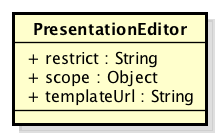
\includegraphics[width=0.4\linewidth]{img/premi_front_end_directives_presentationeditor}
		\caption[Premi::Front-End::Directives::PresentationEditor]{Premi::Front-End::Directives::PresentationEditor}
	\end{figure}
	
	\paragraph{Descrizione}
	Rappresenta il componente grafico che permette all'utente di accedere alla sezione per la modifica di una presentazione.
	
	\paragraph{Utilizzo}
	Viene utilizzata per consentire all'utente di modificare una presentazione. Si attiva quando è selezionato il comando edit nella pagina dei progetti di un utente, deve essere quindi inserita in questa pagina.
	
	\paragraph{Relazione con le altre classi}
	\begin{itemize}
		\item OUT: \textbf{SlideEditor}:\\
		Direttiva che gestisce il componente grafico per la modifica di una \gls{slide}.
	\end{itemize}
	
	\paragraph{Attributi}
	\begin{itemize}
		\item \textbf{+ controller: String}:\\
			Stringa che specifica il controller da associare alla direttiva. Per questa classe è il \textit{PresentationEditorCtrl};
		\item \textbf{+ restrict: String}:\\
			Stringa che specifica la modalità con la quale è possibile inserire la direttiva all'interno della pagina;
		\item \textbf{+ scope: Object}:\\
			Oggetto scope locale della direttiva;
		\item \textbf{+ templateUrl: String}:\\
			Stringa che specifica il percordo dove è situato il file \gls{HTML} che contiene il \gls{template} della direttiva
	\end{itemize}
\newpage


\subsubsection{SlideEditor}
	\begin{figure}[h]
		\centering
		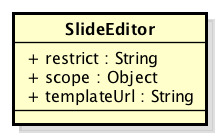
\includegraphics[width=0.4\linewidth]{img/premi_front_end_directives_slideeditor}
		\caption[Premi::Front-End::Directives::SlideEditor]{Premi::Front-End::Directives::SlideEditor}
	\end{figure}
	
	\paragraph{Descrizione}
	Rappresenta il componente grafico che permette all'utente di modificare la \gls{slide} di una presentazione.
	
	\paragraph{Utilizzo}
	Viene utilizzata per consentire all'utente di modificare una \gls{slide} specifica di una presentazione. Si attiva quando viene attivata la direttiva per la modifica di una presentazione. La direttiva \textit{SlideEditor} è inclusa nella componente grafica della direttiva \textit{PresentationEditor}
	
	\paragraph{Relazione con le altre classi}
	\begin{itemize}
		\item IN: \textbf{PresentationEditor}:\\
		Direttiva che gestisce il componente grafico per la modifica di una presentazione.
	\end{itemize}
	
	\paragraph{Attributi}
	\begin{itemize}
		\item \textbf{+ controller: String}:\\
			Stringa che specifica il controller da associare alla direttiva. In questo caso è lo \textit{SlideEditorCtrl};
		\item \textbf{+ restrict: String}:\\
			Stringa che specifica la modalità con la quale è possibile inserire la direttiva all'interno della pagina;
		\item \textbf{+ scope: Object}:\\
			Oggetto scope locale della direttiva;
		\item \textbf{+ templateUrl: String}:\\
			Stringa che specifica il percordo dove è situato il file \gls{HTML} che contiene il \gls{template} della direttiva
	\end{itemize}
\newpage


\subsubsection{Projects}
	\begin{figure}[h]
		\centering
		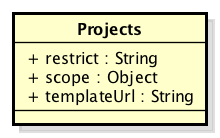
\includegraphics[width=0.4\linewidth]{img/premi_front_end_directives_projects}
		\caption[Premi::Front-End::Directives::Projects]{Premi::Front-End::Directives::Projects}
	\end{figure}
	
	\paragraph{Descrizione}
	Rappresenta il componente grafico che permette all'utente di accedere alla sezione per la visualizzazione dei propri progetti.
	
	\paragraph{Utilizzo}
	Viene utilizzata per consentire all'utente di visualizzare i suoi progetti per poi accedere alle sezioni di presentazione o modifica. Si attiva quando l'utente ha fatto il login e entra nella sua area riservata.
	
	\paragraph{Attributi}
	\begin{itemize}
		\item \textbf{+ controller: String}:\\
			Stringa che specifica il controller da associare alla direttiva. Per questa direttiva è il \textit{ProjectsCtrl};
		\item \textbf{+ restrict: String}:\\
			Stringa che specifica la modalità con la quale è possibile inserire la direttiva all'interno della pagina;
		\item \textbf{+ scope: Object}:\\
			Oggetto scope locale della direttiva;
		\item \textbf{+ templateUrl: String}:\\
			Stringa che specifica il percordo dove è situato il file \gls{HTML} che contiene il \gls{template} della direttiva
	\end{itemize}
\newpage


\subsubsection{User}
	\begin{figure}[h]
		\centering
		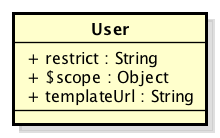
\includegraphics[width=0.4\linewidth]{img/premi_front_end_directives_user}
		\caption[Premi::Front-End::Directives::User]{Premi::Front-End::Directives::User}
	\end{figure}
	
	\paragraph{Descrizione}
	Rappresenta il componente grafico che permette all'utente di accedere alla sezione per la visualizzazione dei propri dati.
	
	\paragraph{Utilizzo}
	Viene utilizzata per consentire all'utente di visualizzare i propri dati. Si attiva nel momento in cui viene eseguito il login al sito.
	
	\paragraph{Attributi}
	\begin{itemize}
		\item \textbf{+ restrict: String}:\\
			Stringa che specifica la modalità con la quale è possibile inserire la direttiva all'interno della pagina;
		\item \textbf{+ scope: Object}:\\
			Oggetto scope locale della direttiva;
		\item \textbf{+ templateUrl: String}:\\
			Stringa che specifica il percordo dove è situato il file \gls{HTML} che contiene il \gls{template} della direttiva
	\end{itemize}
\newpage
